\section{
% Why Model Sparsity for {\MU}?
Model Sparsity: A Missing Factor Influencing Machine Unlearning
}
\label{sec: sparsityMU}

%\SL{[I stop here.]}

%This section shows that model sparsity is a missing factor influencing {\MU}.

%explore the effect of model sparsity (achieved by weight pruning) on {\MU}, demonstrating how  pruning can improve   unlearning in   theory and practice.




\noindent \textbf{Model sparsification via weight pruning.}
% Weight pruning promotes model  sparsity by
% %aims to reduce model sizes by 
% removing  redundant model parameters.
% %\textit{i.e.}, promoting model  sparsity.
% As shown in many prior studies \cite{han2015deep, blalock2020state,chen2021lottery,frankle2018lottery,frankle2020linear,ma2021sanity,zhang2022advancing},  
Model sparsification could not only facilitate  a model's training, inference, and deployment  but also benefit model's performance. For example, LTH (lottery ticket hypothesis) \cite{frankle2018lottery} stated that a trainable sparse sub-model  could be identified from the original dense model, with test accuracy on par or even better than the original model. 
%\PS{This para has lot of overlap with the first para of page 2, including description of LTH. Can be shortened.}
% There also exist many ways to find the desired sparse models,  ranging from pruning at random initialization before training \cite{tanaka2020pruning,frankle2020pruning} to pre-trained weights-based magnitude pruning \cite{ma2021sanity,frankle2018lottery}.
\textbf{Fig.\,\ref{fig: OMP_results}} shows an example of  the pruned model's generalization   vs. its   sparsity ratio. Here  one-shot magnitude pruning (\textbf{OMP}) \cite{ma2021sanity} is adopted to obtain sparse models. 
OMP is computationally the lightest pruning method, which   directly prunes the model weights to the target sparsity ratio based on their magnitudes. As we can see, there exists a graceful sparse regime  with lossless testing accuracy.
%the generalization performance of three commonly-used weight pruning methods 

\iffalse 
\begin{table}[h]
\caption{\footnotesize{OMP trajectory given by test accuracy (\%) VS. sparsity (\%) of ResNet-18 on CIFAR-10 dataset. \SL{Still needs improvement.}}}
\resizebox{0.45\textwidth}{!}{
\begin{tabular}{c|c|c|c|c|c|c|c}
\toprule
   Sparsity  & 0 & 50 & 75 & 90 &95&99&99.5  \\
   \midrule
     \TA& 94.57 & 94.83&94.73&94.76&94.24&92.28&90.05 \\
     \bottomrule
\end{tabular}}
\label{tab: OMP_results}
\end{table}
\fi 
% \begin{figure}[htb]


\begin{wrapfigure}{r}{45mm}
\vspace*{-5mm}
%\vspace*{-6mm}
\centerline{
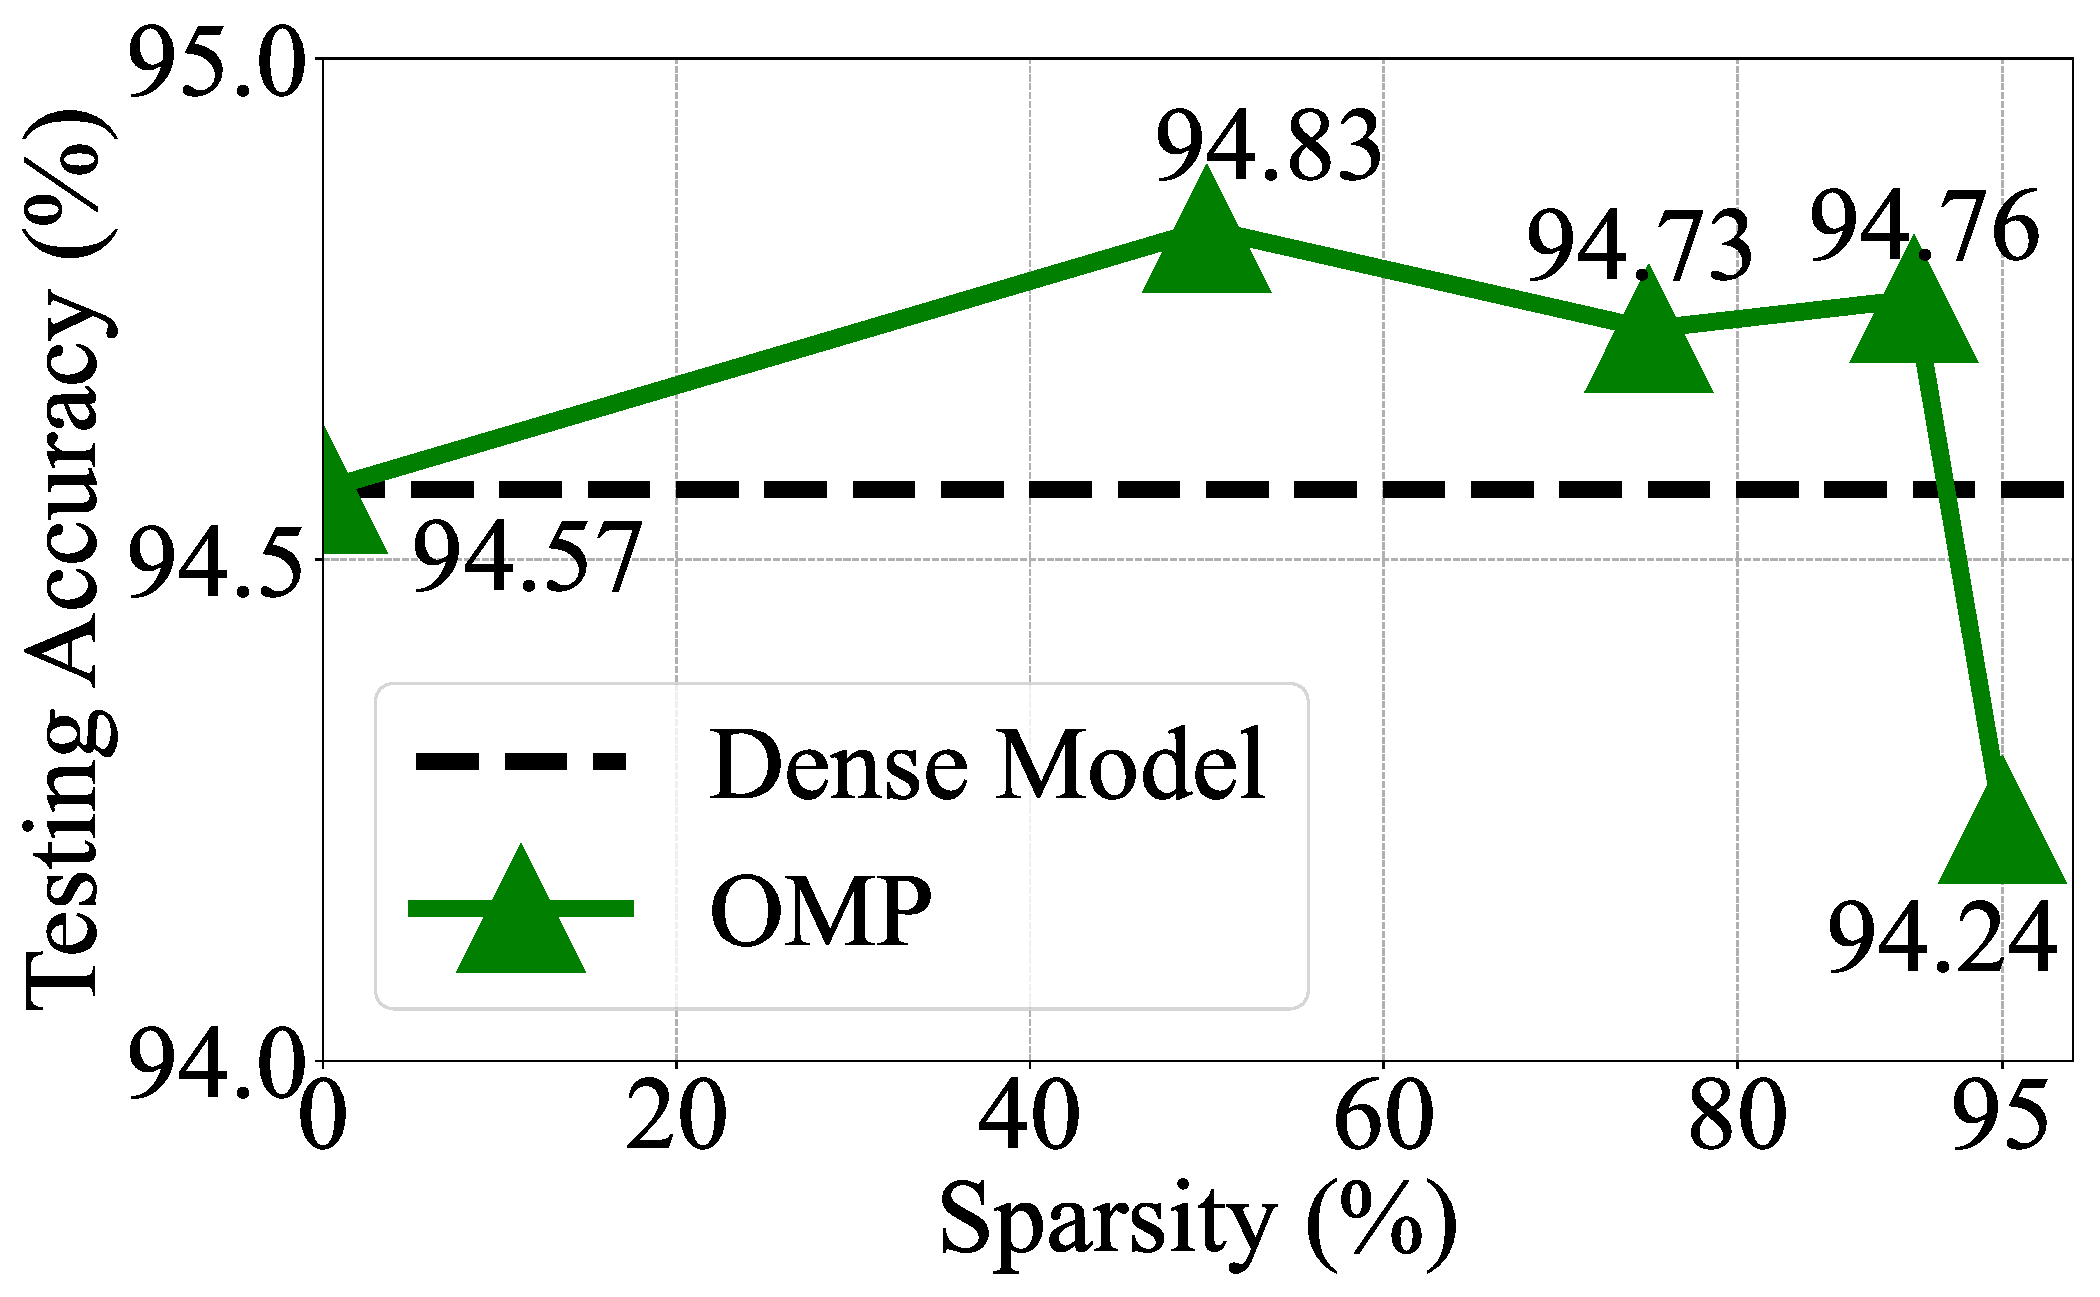
\includegraphics[width=45mm,height=!]{figs/OMP_on_CIFAR-10_ResNet18.pdf}
}
\vspace*{-2mm}
\caption{\footnotesize{
{Testing accuracy  of   OMP-based sparse ResNet-18   vs. the   dense model on CIFAR-10. 
%The  line  represents the mean  of test accuracies over 5 independent trials.
}
}}
  \label{fig: OMP_results}
 \vspace*{-5mm}
\end{wrapfigure}
\noindent \textbf{Gains of {\MU} from sparsity.}
We first analyze the impact of model sparsity on {\MU}  through a lens of   \textit{unrolling stochastic gradient descent} (\textbf{SGD}) \cite{thudi2021unrolling}. The specified SGD method allows us to derive the \textit{unlearning error} (given by the  weight difference between the approximately unlearned model   and the
gold-standard retrained model)  when scrubbing a single data point. However, different from \citet{thudi2021unrolling}, we  will infuse the model sparsity into  SGD unrolling. 


Let us assume a binary mask $\mathbf m$ associated with the model parameters $\btheta$, where $m_i = 0$ signifies that the $i$th parameter 
 $\theta_i$ is pruned to zero and $m_i = 1$  represents the unmasked   $\theta_i$.  This sparse pattern $\mathbf m$ could be obtained by a weight pruning method, like OMP. 
 %in Fig.\,\ref{fig: OMP_results} 
 %\PS{why refer to fig 2 here?}. 
Given $\mathbf m$,   the \textbf{sparse model}  is $ \mathbf m \odot \btheta $, where $\odot$ denotes the element-wise multiplication. Thudi \emph{et al.}\,\cite{thudi2021unrolling} showed that if 
%$\btheta^\prime = \btheta$ (\textit{i.e.}, $\mathbf{m} = \mathbf 1$) and  
{\GA} is adopted to scrub a single data point for the original (dense) model $ \btheta$ (\textit{i.e.}, $\mathbf{m} = \mathbf 1$),  then  the gap between {\GA} and {\retrain} can be approximately bounded in the weight space. 
  \textbf{Prop.\,\ref{prop: SGD_sparse_MU}} extends the existing unlearning error analysis   to a    sparse model. 

%error $e$ (\textit{i.e.}, the  weight difference from  {\retrain}) can be  bounded by

\iffalse 
\vspace*{-5mm}
{\small \begin{align}
   \hspace*{-2mm} e(\btheta_0, \{ \hat{\mathbf z}_i \},  t, \eta) 
 %\nonumber \\
=  \eta^2 \sum_{i=1}^{t-1} [ \nabla_{\btheta,\btheta}^2\ell(\btheta_0, \hat{\mathbf z}_i ) \sum_{j=0}^{i-1}   \nabla_{\btheta} \ell(\btheta_0, \hat{\mathbf z}_j ) ],
 \hspace*{-3mm}
 \label{eq: err_MU_SGD}
\end{align}}%
where $\btheta_0$ is  model initialization when using SGD-based ERM training,    $\{ \hat{\mathbf z}_i \}$
is the sequence of stochastic data samples, $t$ is the number of training iterations, $\eta$ is the learning rate, $\nabla_{\btheta,\btheta}^2\ell(\btheta_0, \hat{\mathbf z}_j)$ is the stochastic Hessian of the training loss $\ell$ evaluated at $\btheta_0$ and the  sample $\hat{\mathbf z}_j$.
Built upon \eqref{eq: err_MU_SGD}, 
%In the following 
Prop.\,\ref{prop: SGD_sparse_MU}  shows the    unlearning error   of {\GA} on a sparse model.
\fi 

%\SL{[Updated prop. Please check.]}
\begin{myprop}
\label{prop: SGD_sparse_MU}
Given the model sparse pattern $\mathbf m$ and the SGD-based  training, the unlearning error   of  {\GA}, denoted by $e(\mathbf m)$, can be characterized by the weight distance
between the {\GA}-unlearned model and the gold-standard retrained model. This leads to the error bound
\iffalse 
and 
 \underline{$ e_{\Omega_{\mathbf m}}(\btheta_0, \{ \hat{\mathbf z}_i \},  t, \eta) $}, where
 $e_{\Omega_{\mathbf m}}$ 
signifies the subvector of $e$ in \eqref{eq: err_MU_SGD} with coordinates given by the unmasked index set $\Omega_m$,  and $\Omega_{\mathbf{m}} = \{ i: m_i = 1 \}$ is the index set of unmasked parameters.
\fi 
%
% \vspace*{-5mm}
% {\small\begin{align}
%   \|  e^\prime(\btheta_0^\prime, \{ \hat{\mathbf z}_i \},  t, \eta)  \|_2 =
%   \|  e_{\Omega_{\mathbf m}}(\btheta_0, \{ \hat{\mathbf z}_i \},  t, \eta) \|_2 ,
%   \label{eq: MU_err_m}
% \end{align}}
% where $\btheta_0^\prime = \mathbf m \odot \btheta_0$,
% $\Omega_{\mathbf{m}} = \{ i: m_i = 1 \}$ is the index set of unmasked parameters, {\color{cyan}and  $e_{\Omega_{\mathbf m}}$ refers to the subvector of $e$ in \eqref{eq: err_MU_SGD} with coordinates given by the unmasked index set $\Omega_m$.}
%
%And the Euclidean norm of the unlearning error can be approximately bounded by
%modifies \eqref{eq: err_MU_SGD} to 
%\begin{align}
\iffalse
  $  e^\prime(\btheta_0^\prime, \{ \hat{\mathbf z}_i \},  t, \eta) \Def \mathbf m \odot e(\btheta_0, \{ \hat{\mathbf z}_i \},  t, \eta) $, where $e$ is  defined in  \eqref{eq: err_MU_SGD}.  
  \fi 
%\end{align}
%$\mathbf m \odot e(\btheta_0, \{ \hat{\mathbf z}_i \},  t, \eta) $. 
%an approximate     upper bound of the above  error is  given by
% \begin{align}
%     e(\mathbf m, \btheta_0, \{ \hat{\mathbf z}_i \},  t, \eta) 
% \end{align}

\vspace*{-5mm}
{\small\begin{align}
  % \|   e_{\Omega_{\mathbf m}}(\btheta_0, \{ \hat{\mathbf z}_i \},  t, \eta)  \|_2 
  e(\mathbf m) = \mathcal{O}(\eta^2 t  \| 
   \mathbf m \odot (\btheta_t - \btheta_0) \|_2 \sigma(\mathbf m) )
  % \leq \frac{\eta}{2}{(t-1) \|    \mathbf m \odot (\btheta_t - \btheta_0) \|_2}  \sigma(\mathbf m),
   \label{eq: err_bd_SGD_sparse}
\end{align}}%
where $\mathcal O$ is the big-O notation, $\eta$ is the learning rate, 
$t$ is the number of   training iterations, 
$ (\btheta_t - \btheta_0)$ denotes the weight difference at iteration $t$ from its   initialization $\btheta_0$,  and
$\sigma(\mathbf m)  $ is the largest singular value ($\sigma$) of the  Hessian $\nabla_{\btheta,\btheta}^2\ell$ (for a training loss $\ell$)   among the  unmasked parameter dimensions, \textit{i.e.}, $\sigma(\mathbf m) \Def \max_{j} \{  \sigma_{j}( \nabla_{\btheta,\btheta}^2\ell ), \text{if } m_j \neq 0  \}$.
%Here   $\sigma_j (\mathbf A)$ is the $j$th singular value of a matrix $\mathbf A$.

\textbf{Proof}: 
See Appendix\,\ref{appendix: SGD_sparse_MU}. 
%\SL{[ @Pranay, @Jinghan, @Jiancheng. Please check and use the above notations to complete the proof in appendix]}
\hfill $\square$
\end{myprop}
% \begin{myprop}
% \label{prop: SGD_sparse_MU}
% Given the model sparse pattern $\mathbf m$ and the SGD-based  training over the non-zero model weights in $\btheta^\prime$, the unlearning error of   {\GA} to scrub a single data point yields
% %modifies \eqref{eq: err_MU_SGD} to 
% %\begin{align}
%   $  e^\prime(\btheta_0^\prime, \{ \hat{\mathbf z}_i \},  t, \eta) \Def \mathbf m \odot e(\btheta_0, \{ \hat{\mathbf z}_i \},  t, \eta) $, where $e$ is  defined in  \eqref{eq: err_MU_SGD}.  
% %\end{align}
% %$\mathbf m \odot e(\btheta_0, \{ \hat{\mathbf z}_i \},  t, \eta) $. 
% An approximate     upper bound of the above  error is  given by
% % \begin{align}
% %     e(\mathbf m, \btheta_0, \{ \hat{\mathbf z}_i \},  t, \eta) 
% % \end{align}
% \begin{align}
%    \|   e^\prime(\btheta_0^\prime, \{ \hat{\mathbf z}_i \},  t, \eta)  \|_2 \leq \frac{\eta (t-1) \| \btheta_t - \btheta_0 \|_2}{2}  \sigma(\mathbf m),
%    \label{eq: err_bd_SGD_sparse}
% \end{align}
% where $\sigma(\mathbf m)  $ is the largest singular value of the stochastic Hessian $\nabla_{\btheta,\btheta}^2\ell$ given in \eqref{eq: err_MU_SGD} among the  model dimensions unpruned, \textit{i.e.}, $\sigma(\mathbf m) \Def \max_{j} \{  \sigma_{j}( \nabla_{\btheta,\btheta}^2\ell ), \text{if } m_j \neq 0  \}$. Here   $\sigma_j (\mathbf A)$ denotes the $j$th singular value of the matrix $\mathbf A$.
% \end{myprop}
We next draw some key insights   from \textbf{Prop.\,\ref{prop: SGD_sparse_MU}}. \textit{First},  it is clear from  \eqref{eq: err_bd_SGD_sparse} that the unlearning error reduces as the model sparsity in $\mathbf m$ increases. 
By contrast, the unlearning error  derived in  \citet{thudi2021unrolling} for a  dense model  (\textit{i.e.}, $\mathbf{m} = \mathbf 1$) is proportional to the dense model distance $\| \btheta_t - \btheta_0 \|_2$. 
%yields $O(\eta^2 t \| \mathbf{w}_t - \mathbf w_0 \|_2 \sigma(\mathbf 1))$.
%Recall that this unlearning error is given by the distance from the exact unlearned model.   
Thus,   model sparsity  is beneficial to reducing the gap between ({\GA}-based) approximate and exact unlearning. 
\textit{Second}, the error bound \eqref{eq: err_bd_SGD_sparse}  enables us to relate {\MU} to the  spectrum of the  Hessian  of the loss landscape. 
%Proposition\,\ref{prop: SGD_sparse_MU} that  the error term $\sigma(\mathbf m)$ in \eqref{eq: err_bd_SGD_sparse} characterizes the influence of model sparsity in {\MU}.  First, 
The number of active singular values (corresponding to nonzero dimensions in $\mathbf m$) decreases when the sparsity grows.
However, it is important to note that in a high-sparsity regime, the model's generalization   could   decrease. Consequently, it is crucial to  select the model sparsity to strike a balance between generalization   and unlearning performance.

% \SL{[Needs to clarify not  the sparser the better due to generalization loss.]}
% On the other hand, the magnitudes of these singular values also decrease since weight pruning can reduce the sharpness of the loss landscape; see  supporting  results in \textbf{Fig.\,\ref{fig: singular_sparsity}}.
%\SL{[Let us decide at the end if we should   move this to appendix.]}
%\PS{Is there a way to show this theoretically, since currently, in (4) we only observe decrease in number of active singular values.} 
% Such pruning effect has also been  justified by existing studies, \textit{e.g.},     %the reduced sharpness of the Hessian   \cite{chen2022can} and 
% the linear model connectivity of sparse models   \cite{frankle2020linear}. 
%The aforementioned insights from   \eqref{eq: err_bd_SGD_sparse}  also justify    that the unlearning error decreases as the sparsity of $\mathbf m$ increases; \PS{Isn't the last sentence redundant with first few sentences in this para?}


%Therefore, our key insight  from Proposition\,\ref{prop: SGD_sparse_MU} is that     model sparsity can contribute to reducing the gap between {\GA}-based approximate unlearning and exact unlearning. 

%the   error of  the {\GA}-based approximate unlearning method. 

%if the model is not pruned (\textit{i.e.}, $\mathbf m = \mathbf 1$), then 

%We provide some  insights   drawn from Proposition\,\ref{prop: SGD_sparse_MU} on the influence of model sparsity in {\MU}.  

% \begin{figure}[htb]
% %\begin{wrapfigure}{r}{80mm}
% %\vspace*{-6mm}
% \centerline{
% %\begin{tabular}{cc}
% %\hspace*{0mm}\includegraphics[width=.3\textwidth,height=!]{figure/performance_comparison.pdf}  
% %&
% %\hspace*{-4mm}
% \includegraphics[width=.31\textwidth,height=!]{example-image-a}
% % \\
% % \hspace*{2mm}\footnotesize{(a) Test accuracy vs. pruning ratio.} &   \footnotesize{(b) Runtime of pruning.}
% %\end{tabular}
% }
% \vspace*{-3mm}
% \caption{\footnotesize{
% TBD. 
% }}
%   \label{fig: singular_sparsity}
% %  \vspace*{-3.8mm}
% %\end{wrapfigure}
% %\end{figure}
% \end{figure}


\begin{figure*}[t]
% \vspace*{-3mm}
\centerline{
\begin{tabular}{cccc}
    \hspace*{-2mm}  \includegraphics[width=0.25\textwidth,height=!]{figs/ua.pdf} &
    \hspace*{-5mm} \includegraphics[width=0.25\textwidth,height=!]{figs/mia.pdf} &
    \hspace*{-5mm} 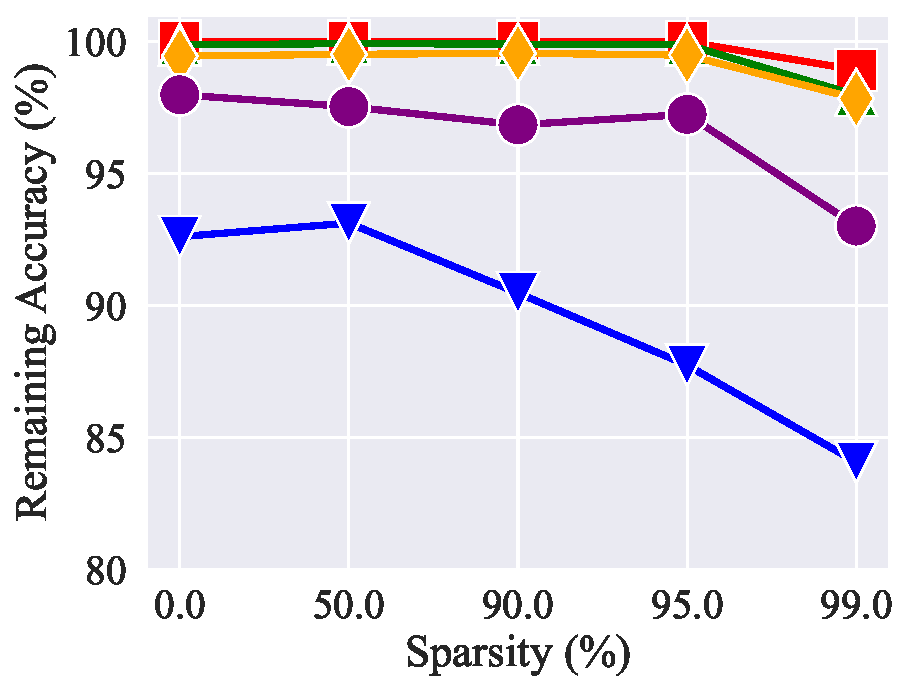
\includegraphics[width=0.25\textwidth,height=!]{figs/ra.pdf} &
    \hspace*{-5mm}  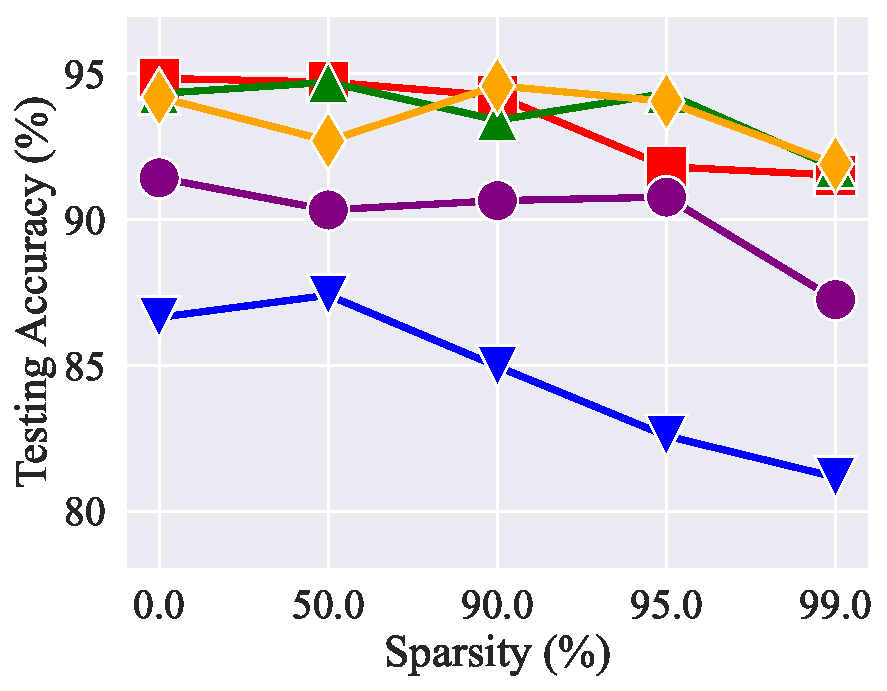
\includegraphics[width=0.25\textwidth,height=!]{figs/ta.pdf} 
\end{tabular}}
 \vspace*{-3mm}
\caption{\footnotesize{
%\SL{[Figure needs updating.]} %\JC{"Retain" -> "Remain"}
Performance of approximate unlearning ({\FTC}, {\GAC}, {\FFC}, {\IUC}) and exact unlearning ({\retrainC}) in efficacy ({\UA} and {\MIAF}), fidelity ({\RA}), and generalization ({\TA}) vs. model sparsity (achieved by {OMP}) in the data-model setup (CIFAR-10, ResNet-18). 
The unlearning scenario is class-wise 
 forgetting, and 
the average unlearning  performance over 10 classes is reported. We remark that being closer to \textcolor{red}{Retrain} performance is better for approximate MU schemes.
% \JC{TODO: Remove legend in fig 3c}
%\PS{See comment in the last para of Section 3. Are we trying to forget an entire class?}
}}
\vspace*{-7mm}
\label{fig: results_OMP_MU}
\end{figure*}

Inspired by Prop.\,\ref{prop: SGD_sparse_MU}, we ask: 
\textit{Does the above   benefit of model sparsification in {\MU} apply to   other approximate unlearning methods besides {\GA}?} This drives us to investigate the performance of approximate unlearning across the entire spectrum as depicted in  {Tab.\,\ref{tab: summary_MU_methods_metrics}}.
%unlearning on sparse models through our   multi-criteria evaluation in \textbf{Tab.\,\ref{tab: summary_MU_methods_metrics}}.
% conduct  the  all-dimension unlearning performance assessment 
% on sparse models, where evaluation metrics have been listed   in Table\,\ref{tab: summary_MU_methods_metrics}. 
Therefore,
\textbf{Fig.\,\ref{fig: results_OMP_MU}} shows the unlearning efficacy ({\UA} and {\MIAF}), fidelity ({\RA}), and generalization ({\TA}) of different   approximate unlearning methods   in the sparse model regime. Here class-wise forgetting is considered for {\MU} and OMP is used for weight pruning. 
% to 
% remove the influence of   all data points in one class from models pruned to different sparsity levels using OMP.
%\PS{We're trying to forget all the points from one class, right? This is not clear from this sentence.}
% on  OMP-based %\PS{``based''?}
% sparse models at different sparsity ratios. \PS{How about: ``... to remove the influence of all the data points belonging to a particular class from models pruned to different sparsity levels using OMP.''?}
%The performance of exact unlearning via {\retrain} is   provided for comparison. 
As we can see, the efficacy of approximate unlearning is significantly improved as the model sparsity increases, \textit{e.g.},   {\UA} and {\MIAF} of using {\FT} over 90\% sparsity.  By contrast, {\FT} over the dense  model (0\% sparsity) is the least effective for {\MU}. 
%\PS{Why do we mention FT alone? The same conclusion seems to hold for GA, FF, IU as well.}
%We also note that the efficacy  of {\retrain} is resilient to model sparsity. 
Also, the efficacy gap between exact unlearning ({\retrain}) and  approximate unlearning  reduces on sparse models. Further, through the fidelity and generalization lenses, {\FT} and {\FF} yield the {\RA} and {\TA}  performance closest to {\retrain}, compared to other unlearning methods. In the regime of ultra-high  sparsity (99\%), 
the efficacy of unlearning exhibits a tradeoff with  {\RA} and {\TA} to some extent.   
%For example, at the $95\%$-sparsity  regime, 

% presents our evaluation results  on {OMP}-based sparse models used in Fig.\,\ref{fig: OMP_results}. 
% % empirically study   the performance metrics  of   {\MU} methods  (Table\,\ref{tab: summary_MU_methods_metrics}) when applied to     sparse models given by OMP   in  Fig.\,\ref{fig: OMP_results}. Fig.\,\ref{fig: results_OMP_MU} shows our full-dimension assessments of {\MU} against model sparsity. 
% As we can see, \SL{[list key principled results.]}


% \begin{figure}[htb]
% \vspace*{-3mm}
% \centerline{
% \begin{tabular}{cccc}
%     \hspace*{-5mm}  \includegraphics[width=.23\textwidth,height=!]{figs/ua.pdf} &
%     \hspace*{-5mm} \includegraphics[width=.23\textwidth,height=!]{figs/mia.pdf} \\
    
%     \hspace*{-5mm} 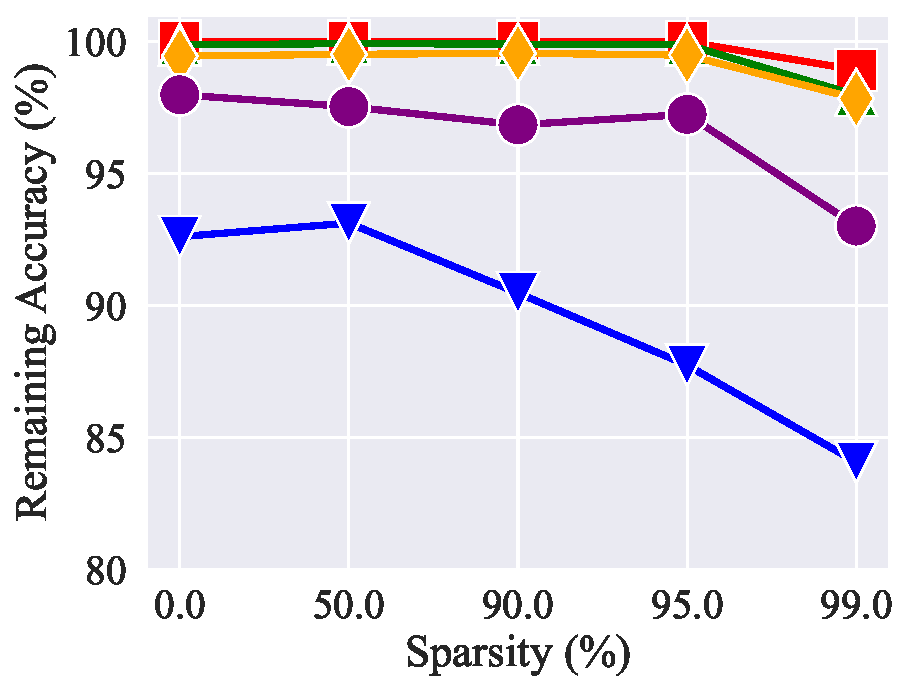
\includegraphics[width=.23\textwidth,height=!]{figs/ra.pdf} &
%     \hspace*{-5mm}  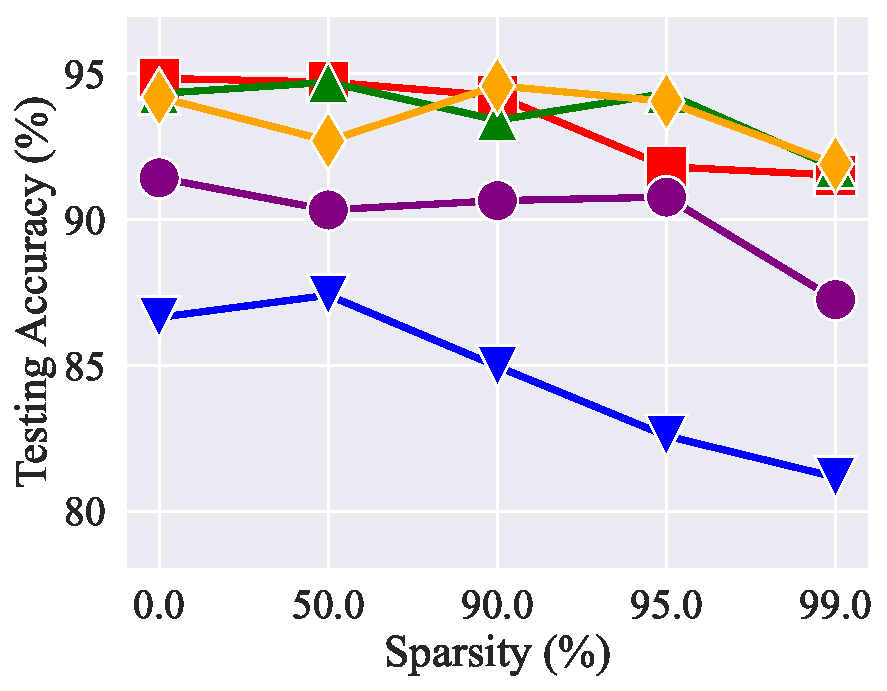
\includegraphics[width=.23\textwidth,height=!]{figs/ta.pdf} 
% \end{tabular}}
%  \vspace*{-3mm}
% \caption{\footnotesize{
% %\SL{[Figure needs updating.]} %\JC{"Retain" -> "Remain"}
% Performance of approximate unlearning ({\FTC}, {\GAC}, {\FFC}, {\IUC}) and exact unlearning ({\retrainC}) in efficacy ({\UA} and {\MIAF}), fidelity ({\RA}), and generalization ({\TA}) vs. model sparsity (achieved by {OMP}) in the data-model setup (CIFAR-10, ResNet-18). 
% The unlearning scenario is class-wise 
%  forgetting, and 
% the average unlearning  performance over 10 classes is reported. 
% %\PS{See comment in the last para of Section 3. Are we trying to forget an entire class?}
% }}
% % \vspace*{-3mm}
% \label{fig: results_OMP_MU}
% \end{figure}

